\FloatBarrier
\section{Robustness}\label{app:robustness}\setcounter{equation}{0}
Figure \ref{fig:robustness} sets the paper's main results against the specifications behind them, one panel per result. With the pension design given, the panels are the change in the equilibrium tax rate from $\theta = 1$ to $\theta = 0$ and under acute ageing, France's income distribution and France's voting patterns, in percentage points; with the design chosen, they are the change in the chosen design under the same three counterfactuals. Each marker is one specification, read in 2020 against the host economy's own baseline at the same $\rho$: its colour is the intertemporal elasticity, its shape the calibration of the taste for leisure, common $X$ or vector $X_i$ (\oa{oecd-vectorx}), and its row group the host economy. For the chosen design, which is solved under a common $X$ only, further rows hold the alternative cost of the \oa{esc-scale}, the UK as host under France's characteristics and, under acute ageing at $\rho = 1$, the Frisch elasticities $\xi = 0.2$ and $0.4$. The paper's own reading, the U.S.\ under a common $X$ at $\rho = 1$ with the cost of section \ref{sec:esc:cost}, is highlighted, and a line marks zero: the spread of a panel's markers around the highlighted one is how far the result depends on the specification, and a marker on the other side of the line is a change of sign. The online appendix at \oahome is organized around this figure and links each marker to the table and the row that print its value.

\begin{figure}[!htb]
    \centering
    \caption{The main results across specifications}
    \label{fig:robustness}
\begin{threeparttable}
    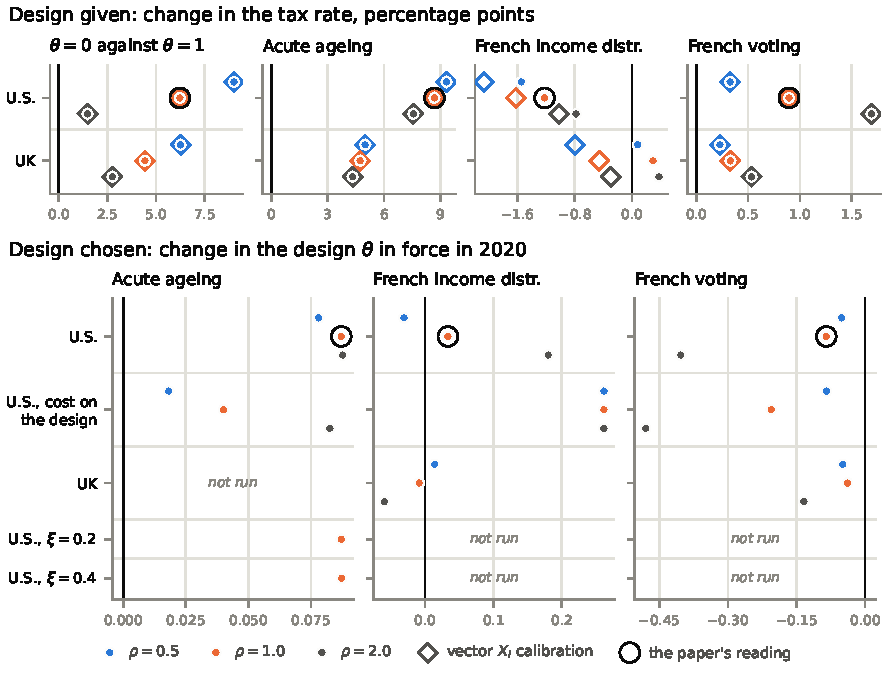
\includegraphics[width=\linewidth]{Figs/RobustnessMap.pdf}\par
\begin{tablenotes}[flushleft]\footnotesize
    \item[] \textit{Note:} Every value is read in 2020. Table \ref{table:US_ESC:summary} prints the designs chosen for the U.S.\ under a common $X$ with the cost of section \ref{sec:esc:cost}; every other value is printed in the online appendix, sections \oanum{oecd-us} and \oanum{oecd-uk} with the design given and \oanum{esc-us} and \oanum{esc-uk} with it chosen.
\end{tablenotes}
\end{threeparttable}
\end{figure}
